\begin{figure}[t]
\centering
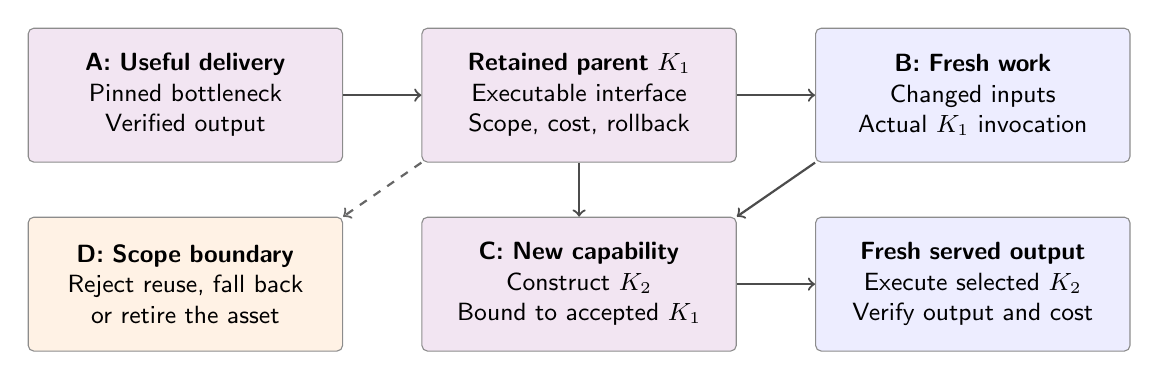
\begin{tikzpicture}[
  font=\sffamily\small,
  box/.style={draw=black!45, rounded corners=2pt, align=center, text width=3.5cm, minimum height=1.7cm, inner sep=7pt},
  flow/.style={->, thick, draw=black!70},
  guard/.style={->, thick, dashed, draw=black!60}
]
\node[box,fill=violet!10] (a) at (0,0) {\textbf{A: Useful delivery}\\Pinned bottleneck\\Verified output};
\node[box,fill=violet!10] (k) at (5,0) {\textbf{Retained parent $K_1$}\\Executable interface\\Scope, cost, rollback};
\node[box,fill=blue!7] (b) at (10,0) {\textbf{B: Fresh work}\\Changed inputs\\Actual $K_1$ invocation};
\node[box,fill=violet!10] (c) at (5,-2.4) {\textbf{C: New capability}\\Construct $K_2$\\Bound to accepted $K_1$};
\node[box,fill=blue!7] (serve) at (10,-2.4) {\textbf{Fresh served output}\\Execute selected $K_2$\\Verify output and cost};
\node[box,fill=orange!10] (d) at (0,-2.4) {\textbf{D: Scope boundary}\\Reject reuse, fall back\\or retire the asset};
\draw[flow] (a) -- (k);
\draw[flow] (k) -- (b);
\draw[flow] (k) -- (c);
\draw[flow] (b.south west) -- (c.north east);
\draw[flow] (c) -- (serve);
\draw[guard] (k.south west) -- (d.north east);
\end{tikzpicture}
\caption{Artifact lineage and failure boundary. A useful delivery, fresh reuse and construction of a distinct capability are separate achievements. The child must be tied to accepted parent bytes, and the selected child must actually use them when required by the claimed mechanism. Scope failure preserves the history while ending the invalid reuse claim.}
\label{fig:lineage}
\end{figure}
